%!TEX root = main.tex


\section{Introduction}\label{sec:intro}

The number of reported security breaches due to \emph{virus}, \emph{worms}, \emph{trojans}, etc, has been growing considerably in recent years~\cite{av-test:report} with reports of infections due to \emph{malware}  making the headlines, now more than ever.
Almost every week one such security vulnerability is reported which may be seen as a failure by the security community on the control and detection of malicious content. 

The very first challenge that we face is the definition of \emph{malware}.
Malware is considered to be \say{a program with malicious intent}~\cite{christodorescu:semantics} which in itself is a dubious definition. 
Not only the same programs are classified differently as \emph{malware} and \emph{goodware} depending on the vendor, but also some programs fall within a gray area for which no clear classification can be deemed correct.
An example is what is called \emph{adware}, advertising-supported software, that although not performing directly malicious actions, perform arguably non-requested actions.
The non-existence of concrete metrics and properties that uniquely distinguish malware from goodware requires an extra effort in the preparation of datasets for evaluation of malware detectors.

Due to the significant number of malware attacks, and taking into consideration the increasing popularity and huge success of \gls{ml} methodologies in classification in different domains~\cite{lee2003learning,joachims2002learning,li2010object,ding2001multi}, it is only natural to see these techniques applied to complement classical methodologies for malicious-content detection~\cite{arp2014drebin,christodorescu:semantics,kolosnjaji2016deep,kolter:learning,miller:rev_int,nissim:al_pdf,perdisci:behavior,rieck:dynamic,santos2013opcode,schultz:data_mining,schwenk2012autonomous,vsrndic2013detection,deo2016prescience,gandotra2014malware,jordaney2017transcend,rossow:practices}, in particular, supervised learning techniques.
However, several issues have arised regarding the usage of these ML techniques in the scope of malware analysis~\cite{deo2016prescience,gandotra2014malware,jordaney2017transcend,rossow:practices}.

On the sometimes ambiguous scenario that is the task of distinguishing malware from goodware, some of these results largely depend on the datasets used for evaluation, often not representing the real-world. 
In this paper we address this pertinent questions and make a comparative analysis of a supervised learning approach in three different scenarios (depicted in Figure~\ref{fig:scenarios}): a \emph{strict scenario} where only very well-characterized samples are considered, a \emph{loose scenario} where a wider set of still well-studied samples is considered, and finally a \emph{realistic scenario} where we get closer to the reality faced by vendors of malware detection solutions.

\begin{figure}[!h]
	\centering
	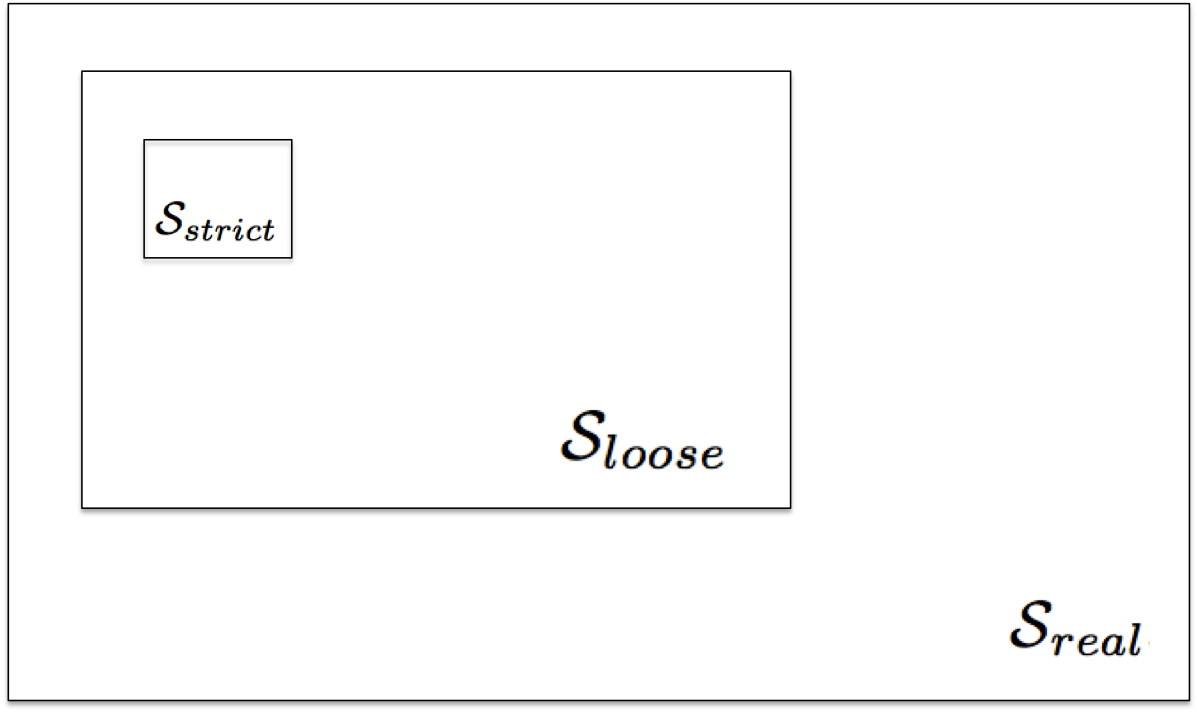
\includegraphics[width=2.5in]{dataset_sizes}
	\caption{Representation of our $\mathcal{S}_{strict}$, $\mathcal{S}_{loose}$ and $\mathcal{S}_{real}$ scenarios.}
	\label{fig:scenarios}
\end{figure}

Throughout this work we will perform a comparative analysis of the three above scenarios under two distinct environments:

\begin{itemize}[noitemsep]
	\item \emph{laboratory conditions} where traditional cross-validation methodologies can be applied;
	\item \emph{real-world conditions} where time is relevant and we analyze the behavior of the classifier with temporal-based methodologies.
\end{itemize}

We show that without much tweaking, and using simple features, a \gls{lr} model is able to achieve an \gls{auroc} of 0.91 when ideal laboratory conditions are met, but these results go down to an \gls{auroc} of 0.75 when we change into a real-world scenario.

With the purpose of actually evaluating the usage of \gls{ml} methodologies for malware detection as a complement to traditional malware detection techniques, we also analyze how the size of the training set can influence the performance of the classifier under the three studied scenarios.
For this, we use the aforementioned temporal-based methodologies to come up with conclusions on how large the training set need to be to ensure optimal results from the classifier.

We finish off by improving our base model to include more dynamic features, as well as providing a multi layer approach which adds the ability of classifying malware samples from different classes, in contrast with simply providing if a sample is malware or not.
These improvements boost our \gls{auroc} to 0.98 in ideal laboratory conditions and 0.95 in a real-world scenario.

As the main contributions of this paper
\begin{enumerate*}[label={\alph*)},font={\color{red!80!black}\bfseries}]
	\item we propose three different scenarios to train and validate the model which range from a more simulated scenario to a more realistic one,
	\item temporal-based methodologies to train and validate the classifier, 
	\item we study how much can we reduce the training dataset without compromising the optimal results,
	\item we improve our base model by 7\% to 27\%.

\end{enumerate*}


This paper is outlined as follows: in Section~\ref{sec:related} we present
the related work and justify how it motivated our work; in Section~\ref{sec:data} we describe and analyze the available dataset and how it was labeled; in Section~\ref{sec:feature_model} we propose a feature selection and describe the used model; Section~\ref{sec:eval_results} encloses our main contributions, describing our three scenarios and how they are to be evaluated, using regular cross-validation and our defined temporal-based methodology, together with the results of said evaluation;
in Section~\ref{sec:improvements} we provide improvements to our base model; in Section~\ref{sec:discussion} we discuss our main achievements; Section~\ref{sec:conclusion} concludes the paper and discusses avenues for further research.
